\documentclass[addpoints]{exam}
\usepackage[utf8]{inputenc}
\usepackage{amsmath}
\usepackage{mathtools}
\usepackage{tikz}
\usepackage{pgfplots}
\usetikzlibrary{datavisualization}
\usetikzlibrary{datavisualization.formats.functions}
\usepackage{relsize}
\usepackage{dirtytalk}
\usepackage{graphicx}
\graphicspath{ {./drift/} }
\DeclarePairedDelimiter{\ceil}{\lceil}{\rceil}
\usepackage{geometry}
\usepackage{draftwatermark}
\SetWatermarkFontSize{2cm}
\SetWatermarkText{$2^{77,232,917}-1$}
\usepackage[banglamainfont=Kalpurush, 
            banglattfont=Siyam Rupali
           ]{latexbangla}
        
\begin{document}
\begin{LARGE}
\begin{center}
গণিত (Mathematics - 2002)
\end{center}
\end{LARGE}
\begin{questions}

\question  $ \sin 65^{\circ} + \cos 65^{\circ} $ সমান- (equals)

\begin{oneparchoices}
\choice $ \dfrac{\sqrt{3}}{2}\cos 40^{\circ} $
\choice $ \dfrac{1}{2}\sin 20^{\circ} $
\choice $ \sqrt{2}\cos 20^{\circ} $
\choice $ \dfrac{\sqrt{3}}{2}\sin 40^{\circ} $
\end{oneparchoices}

\question  (What is the co efficient in the expansion of ) $ \Big(a+\dfrac{1}{a}\Big)^{18} $  এর বিস্তৃতিতে $ a^{0} $ এর সহগ কত? 

\begin{oneparchoices}
\choice  48620
\choice  38620
\choice  48640
\choice  48720
\end{oneparchoices}

\question (The slope of the tangent drawn at the point $ (-1,1) $ on the curve) $ 3x^{2}-7y^{2}+4xy-8x=0 $ বক্ররেখাটির $ (-1,1) $ বিন্দুতে অঙ্কিত স্পর্শকের ঢাল- (is)

\begin{oneparchoices}
\choice $ -\dfrac{5}{9} $
\choice $ \dfrac{5}{9} $
\choice $ -\dfrac{9}{5} $
\choice $ \dfrac{9}{5} $
\end{oneparchoices}



\question $ (-1,1) $  বিন্দুগামী এবং $ 2x-3y+6=0 $ রেখার উপর লম্ব সরলরেখার সমীকরণ- (The equation of the straight line through the point $ (-1,1) $ and perpendicular to the line $ 2x-3y+6=0 $ is) 

\begin{oneparchoices}
\choice $ 3y-2x=-5 $
\choice $ 3x+2y=-1 $
\choice $ 2y-3x=1 $
\choice $ 3x+2y=1 $
\end{oneparchoices}

\question  (If) $ \begin{pmatrix}
x-y & 1\\
7 & x+y
\end{pmatrix} = \begin{pmatrix}
8 & 1\\
7 & 2
\end{pmatrix} $ হলে (then) $ (x,y)=? $ 

\begin{oneparchoices}
\choice $ (-5,-3) $
\choice $ (5,-3) $
\choice $ (-5,3) $
\choice $ (5,3) $
\end{oneparchoices}

\question নিচের কোন রাশিমালাটি $ \cos 3A $ কে $ \sin A $ বা $ \cos A $ এর বহুপদী রুপে প্রকাশ করে (Which of the following expression gives  $ \cos 3A $ as a polynomial in $ \sin A $ or $ \cos A $) -

\begin{oneparchoices}
\choice  $ 3\cos A -4\cos^{3} A $
\choice  $ 3\sin A -4\sin^{3} A $
\choice  $ 4\cos^{3} A -3\cos A $
\choice  $ 4\sin^{3} A -3\sin A $
\end{oneparchoices}

\question দশমিক সংখ্যা 123 কে দ্বিমিক পদ্ধতিতে প্রকাশ করলে হয়- (The decimal number 115 when expressed in the binary system is )

\begin{oneparchoices}
\choice 1110111
\choice 1111011
\choice 1110110
\choice 1101111
\end{oneparchoices}

\question এক প্যাকেট তাস থেকে একটি তাস দৈবভাবে নেয়া হলো। তাসটি হরতন বা চিরতন হওয়ার সম্ভবনা কত? (One card is drawn at random from a pack of cards. What is the probability that the card drawn is heart or club ? )

\begin{oneparchoices}
\choice $ \dfrac{1}{2} $
\choice $ 2 $
\choice $ \dfrac{4}{13} $
\choice  $ \dfrac{1}{4} $
\end{oneparchoices}

\question  $ \mathlarger{\int}\dfrac{dx}{x+\sqrt{x}} =? $

\begin{oneparchoices}
\choice $ \ln (\sqrt{x} +x) +c$
\choice $ \tan^{-1}(\sqrt{x}+1)+c $
\choice $ 2\ln (\sqrt{x}+1)+c  $
\choice  $ \tan^{-1}(\sqrt{x}+1)+c $
\end{oneparchoices}

\question  $ \lambda $ এর কোন মানের জন্য  $ 4\hat{i}+2\hat{j}-3\hat{k} $ এবং  $ \lambda\hat{i}-3\hat{j}+2\hat{k} $  ভেক্টরদ্বয় পরস্পর লম্ব হবে? (For what value of $ \lambda $ vector $ 4\hat{i}+2\hat{j}-3\hat{k} $ and $ \lambda\hat{i}-3\hat{j}+2\hat{k} $ are perpendicular to each other?)

\begin{oneparchoices}
\choice $ \dfrac{8}{7} $
\choice $ \dfrac{7}{8} $
\choice $ \dfrac{8}{5} $
\choice  $\dfrac{5}{8} $
\end{oneparchoices}

\question বাস্তব সংখ্যায় $ 0<|x-3|<4 $ অসমতাটির সমাধান সেট – (The solution set of the inequality $ 0<|x-3|<4 $ is)

\begin{oneparchoices}
\choice $ \{x:-1<x<7\} $
\choice $  \{x:-1<x<3\} \cap \{x: 3<x<7\}  $\\
\hspace*{-.3cm}\choice $  \{x:-1\le x \le 7\} $
\choice $  \{x:-1<x<3\} \cup \{x: 3<x<7\}$  
\end{oneparchoices}

\question (If) $ y = \cos (\sqrt{y}) $ হলে তখন (then) $ \dfrac{dy}{dx} = $ 

\begin{oneparchoices}
\choice $ \sin (\sqrt{x}) $
\choice $ -\sin (\sqrt{x}) $
\choice $ -\dfrac{\sin (\sqrt{x})}{\sqrt{x}} $
\choice $ -\dfrac{\sin (\sqrt{x})}{2\sqrt{x}} $
\end{oneparchoices}

\question $ (-9,9) $ এবং $ (5,5) $ বিন্দুদ্বয়ের সংযোজক রেখাংশকে ব্যাস ধরে অংকিত বৃত্তের সমীকরণ- (The equation of the circle having the line segment joining the points $ (-9,9) $ and $ (5,5) $ as its diameter is) 

\begin{oneparchoices}
\choice $ x^{2}+y^{2}-4x+14y = 0 $
\choice $ x^{2}+y^{2}-4x-14y = 0 $\\
\hspace*{-.3cm}\choice $ x^{2}+y^{2}+4x+14y = 0 $
\choice $ x^{2}+y^{2}+4x-14y = 0 $
\end{oneparchoices}

\question $ p $ এর কিরুপ মানের জন্য $ x^{2}+px+1=0 $ সমীকরনটির মূলদ্বয় জটিল হবে? (For what range of values of $ p $ will be the equation $ x^{2}+px+1=0 $ have both its roots complex)

\begin{oneparchoices}
\choice $ -2\le p \le 2 $
\choice $ -4\le p \le 4 $
\choice $ -2< p < 2 $
\choice $ -4\le p < 4 $
\end{oneparchoices}

\question একটি ক্লাশের জন ছাত্র সকলেই ক্রিকেট অথবা ফুটবল উভয়ই খেলে। 75 জন ক্রিকেট খেলে এবং 60 জন ফুটবল খেলে। কতজন উভয়ই খেলে? (All 120 students in a class play cricket or football or both. 75 play cricket and 60 play football. How many play both?)

\begin{oneparchoices}
\choice 13
\choice 15
\choice 25
\choice 23
\end{oneparchoices}

\question   প্রক্ষেপকের ভ্রমণকালে $ T $ আনুভুমিক পাল্লা $ R $ এবং আনুভুমিকের সাথে প্রক্ষেপন কোণ $ \alpha $ হলে $ \dfrac{T^{2}}{R} $ সমান- (If $ T $ is the traveling time of a projectile, $ R $ is its horizontal range and $ \alpha $ is the angle of projection, then $ \dfrac{T^{2}}{R} $ equals )

\begin{oneparchoices}
\choice $ \dfrac{2}{g}\tan \alpha $
\choice $ \dfrac{2}{g}\cot \alpha $
\choice $ \dfrac{g}{2}\tan \alpha $
\choice $ \dfrac{g}{2}\cot \alpha $
\end{oneparchoices}

\question $ 3x+4y=10 $ রেখাটির উপর মুলবিন্দু হতে অংকিত লম্বের দৈর্ঘ্য- (the length of the perpendicular drawn from the origin to the line $ 3x+4y=10 $ is )

\begin{oneparchoices}
\choice $ 2 $
\choice $  \sqrt{2} $
\choice $ 5 $
\choice  $ \sqrt{5} $
\end{oneparchoices}

\question  চারজন পুরুষ ও চয়জন মহিলা হতে চার সদস্য বিশিষ্ট একটি উপকমিটি গঠন করা যেতে পারে, যাতে একজন নির্দিষ্ট পুরুষ সর্বদা অর্ন্তভুক্ত থাকে? (In how many ways can a subcommittee of four persons be formed from amongst four women and six men so that one particular man is always included? )

\begin{oneparchoices}
\choice 504
\choice 210
\choice 126
\choice 84
\end{oneparchoices}

\question  নিচের কোনটি $y=-(x-1)^2$ এর লেখচিত্র? 

\begin{oneparchoices}
 \choice 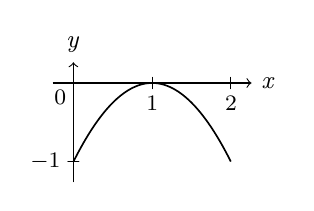
\begin{tikzpicture}
\datavisualization [school book axes,
                    visualize as smooth line,
                    y axis={label},
                    x axis={label} ]

data [format=function] {
      var x : interval [0:2] samples 150;
      func y =  2*\value x -  \value x*\value x - 1 ;
      };
\end{tikzpicture}
 \choice 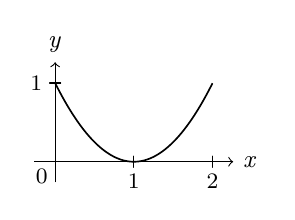
\begin{tikzpicture}
\datavisualization [school book axes,
                    visualize as smooth line,
                    y axis={label},
                    x axis={label} ]

data [format=function] {
      var x : interval [0:2] samples 150;
      func y =   \value x*\value x-2*\value x + 1 ;
      };
\end{tikzpicture}
\choice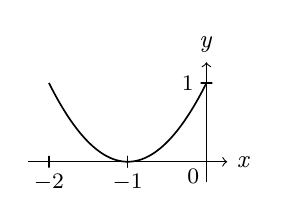
\begin{tikzpicture}
\datavisualization [school book axes,
                    visualize as smooth line,
                    y axis={label},
                    x axis={label} ]

data [format=function] {
      var x : interval [-2:0] samples 150;
      func y =   \value x*\value x+2*\value x + 1 ;
      };
\end{tikzpicture}
 \choice 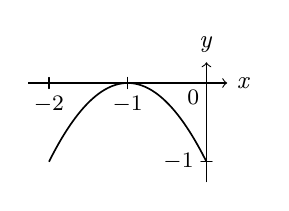
\begin{tikzpicture}
\datavisualization [school book axes,
                    visualize as smooth line,
                    y axis={label},
                    x axis={label} ]

data [format=function] {
      var x : interval [-2:0] samples 150;
      func y =   -\value x*\value x-2*\value x - 1 ;
      };
\end{tikzpicture}
 
\end{oneparchoices}

\question (The value of the determinant) $ \begin{vmatrix}
-8 & 3 & 3\\
3 & -8 & 5\\
5 & 5 & -8
\end{vmatrix} $ নির্নায়কটির মান- 

\begin{oneparchoices}
\choice $ 1 $
\choice $ -1 $
\choice $ 0 $
\choice $ 2 $
\end{oneparchoices}

\question একই বিন্দুতে ক্রিয়ারত 2 একক ও 3 একক মানের দুটি বলের লদ্ধির মান 4 একক। বলদুটির অন্তর্ভুক্ত কোণ কত? (The magnitude of the resultant of two forces acting at a point and having magnitudes 2 units and 3 units. What is the angle between the two forces )

\begin{oneparchoices}
\choice $ \cos^{-1}\Big(\dfrac{1}{4} \Big) $
\choice $ \cos^{-1}\Big(\dfrac{1}{2} \Big) $
\choice $ \cos^{-1}\Big(\dfrac{1}{3} \Big) $
\choice $ \cos^{-1}\Big(\dfrac{1}{5} \Big) $
\end{oneparchoices}

\question  (The value of )  $ \mathlarger{\int_{1}^{e}\ln x\, dx} $ এর  মান (is) – 

\begin{oneparchoices}
\choice  $ e $
\choice  $ e-1 $
\choice  1
\choice  $ 1-e $
\end{oneparchoices}

\question $ \omega $ যদি 1 এর একটি জটিল ঘনমূল হয়, তবে $ (1-\omega +\omega^{2})(1-\omega^{2}+\omega^{4}) $ এর মান – (If $ \omega $ is a complex (imaginary) cube root of unity, thenthe value of $ (1-\omega +\omega^{2})(1-\omega^{2}+\omega^{4}) $ is)
 
\begin{oneparchoices}
\choice $ 4 $
\choice $ 6 $
\choice $ 3 $
\choice $ 2 $
\end{oneparchoices}

\question  নিচের কোন উক্তি সত্য?  (Which of the following statement is true?)

\begin{oneparchoices}
\choice  $ A\setminus B = A\cap B^{\prime} $
\choice  $ A\setminus B = A\cup B^{\prime} $
\choice  $ A\setminus B = A^{\prime}\cap B $
\choice  $ A\setminus B = A^{\prime}\cup B $
\end{oneparchoices}

\question  নিন্মোক্ত রাশিমালার মান-(The value of the following expression $ \sin (780^{\circ})\cos (390^{\circ})-\sin (330^{\circ}) (-300^{\circ})$ )  

\begin{oneparchoices}
\choice $ -1 $
\choice $ 0 $
\choice $ 1 $
\choice $ \dfrac{1}{2} $
\end{oneparchoices}

\end{questions}

\end{document}